\chapter{Analýza problému a existující řešení}
\label{sec:History}

Cílem počítání lidí v obraze je pro vstupní obraz spočítat, nebo co nejpřesněji odhadnout, kolik lidí se v něm celkem nachází.
Ačkoliv jsou dnes pro řešení tohoto problému hojně používány neuronové sítě, historie této disciplíny sahá do doby před nárůstem jejich popularity.
Obecně se používané metody dají rozdělit do tří kategorií a to na přímé (direct), nepřímé (indirect) a metody používající odhad hustotní mapy (density map estimation).

\textbf{Přímé metody} jsou založené na velice intuitivním přístupu k řešení tohoto problému, jímž je detekování jednotlivých lidí nacházejících se ve vstupním obraze. Výsledný počet lidí je u těchto metod roven počtu detekcí. Výkon a přesnost takovéhoto estimátoru jsou tedy silně závislé na výkonu použitého detektoru lidí.
Od toho se také odvíjí nevýhody tohoto přístupu, kdy například v hustě zalidněných scénách často dochází k částečným zakrytím jednotlivých lidí jinými lidmi či objekty, což dělá segmentaci obrazu a následnou detekci lidí v něm výrazně problematičtější.

Do této kategorie by se dal zařadit například estimátor popsaný v článku \cite{head_and_shoulders}.
Vstupní obraz je nejdříve segmentován na popředí a pozadí.
Pro tento účel autoři článku přicházejí s příznakem Mosaic Image Differernce (MID), který funguje tak, že obraz je rozdělen na buňky seskupené do bloků, pro které je vypočítána průměrná barva. Pokud se mezi dvěma po sobě jdoucími snímky v buňce průměrná barva změní více, než jaká je hodnota stanoveného prahu, je blok, ve kterém se nachází, označen jako součást popředí.
Autoři předpokládají, že lidé se v obraze mírně pohybují a proto bude možné tímto způsobem obraz segmentovat.
V segmentovaném obraze jsou poté vyhledáni jednotliví lidé a následně je podle počtu detekcí stanoven jejich počet.
Toho je docíleno pomocí detektoru založeného na metodě sliding window, kdy obsah detekčního okna je popsán příznaky HOG \cite{HOG} a o klasifikaci se stará klasifikátor AdaBoost \cite{AdaBoost}, jenž byl natrénován na obrázcích lidí obsahující jejich hlavy a ramena.

Také by se tady dala zařadit práce \cite{YOLO_counting}, ve které autoři počítají osoby pomocí upravené neuronové sítě YOLO \cite{YOLO}.
Jejich úpravy této sítě spočívaly hlavně v rozdělení obrazu do více buněk a zvýšení počtu bounding boxů počítaných pro každou buňku v obraze. Výslednou síť natrénovali tak, ať je citlivá na lidi.
Počet lidí v obraze byl stanoven jako počet bounding boxů, které se nacházely v oblasti, kterou v obraze vytyčili.
Autoři totiž systém zamýšleli pro použití na počítání lidí vycházejících z eskalátoru nebo na jiných místech, kde si mohli být jisti, že lidé budou procházet úzkým prostorem, který bude blízko kamery snímající scénu, takže jednotliví lidé budou v obraze v okamžiku započítání celkem dobře separováni a budou zabírat velké procento scény.
U scén, kde toto není možné by ale nejspíš tento přístup narážel na stejné problémy, jako jiné přímé metody.


\textbf{Nepřímé metody} vznikly v reakci na problémy přímých metod, které se snaží vyřešit.
Na rozdíl od nich se tedy snaží určit počet lidí v obraze bez nutnosti znalosti pozice každého z nich a místo toho měří jiné veličiny.

Autoři článku \cite{crowd_on_pets} vytvořili estimátor, jenž určoval počet lidí na základě počtu a hustoty příznaků Speeded Up Robust Features (SURF) \cite{SURF} nacházejících se v popředí snímku.
Tento postup je založen na myšlence, že v hustém davu, kde bude docházet k mnoha okluzím, se bude vyskytovat velké množství zájmových bodů, zatímco v případě, kdy jsou lidé ve snímku od sebe izolováni, bude v dané oblasti SURF bodů méně.
O tom, zda příznak patří do popředí, je rozhodnuto na základě vektoru popisujícího pohyb daného zájmového bodu mezi dvěma po sobě jdoucími snímky.
Podobně jako autoři článku \cite{head_and_shoulders}, i zde autoři předpokládají, že i statičtí lidé se mírně pohybují, a proto všechny zájmové body s délkou pohybového vektoru větší, než je nějaký stanovený práh, jsou označeny, že patří lidem.
Oproti metodě z článku \cite{head_and_shoulders}, zde ale nedochází k detekci jednotlivých lidí, a proto bude přesnost tohoto detektoru velice snadno ovlivněna výskytem jiných pohybujících se objektů, které se mohou v obraze nacházet.
Autoři článku se také snaží odstranit negativní účinky perspektivy na přesnost výsledku, a to tím, že blízké zájmové body shlukují do skupin, které ohodnocují zvlášť.
Výsledná funkce, která pro shluk vrátí počet lidí, kteří se v něm nacházejí, je získaná pomocí SVR (Support Vector Regressor) \cite{SVR} a je závislá na počtu bodů ve shluku, jejich hustotě a velikosti ohodnocovaného shluku.

\begin{figure}[h!]
	\centering
	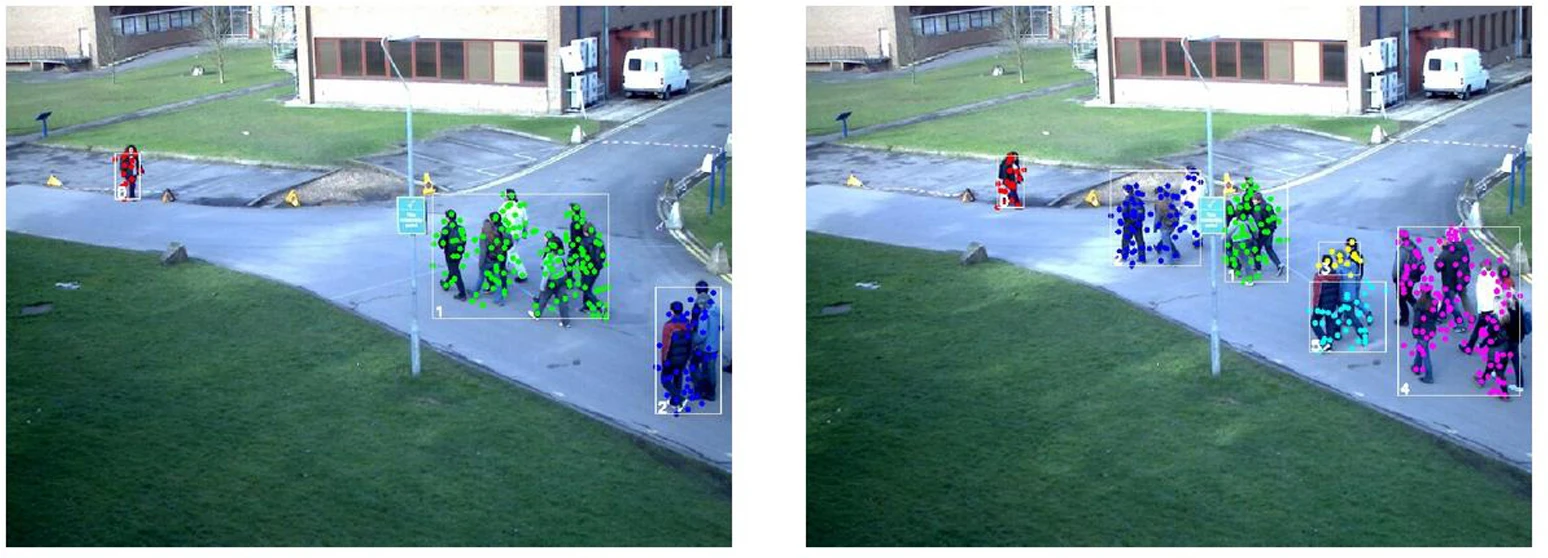
\includegraphics[width=0.8\textwidth]{Figures/history/PETS_CLUSTERS.png}
	\caption{Shlukování SURF bodů metody použité v článku 5 \cite{crowd_on_pets} (převzato z \cite{crowd_on_pets})}
	\label{fig:PETS}
\end{figure}



S narůstající popularitou neuronových sítí v oblasti strojového vidění přirozeně narůstá i množství estimátorů počítajících objekty v obraze, které jsou na neuronových sítích založeny.
S nimi se objevila i nová a dnes velmi často používaná kategorie metod pro počítání objektů v obraze, kterou je počítání lidí pomocí hustotní mapy (Density Map Estimation).

\textbf{Metody používající odhad hustotní mapy} se vyznačují tím, že konvoluční neuronová síť na základě vstupního obrazu vytvoří hustotní mapu, která popisuje odhadovanou hustotu davu v obraze, a výsledný počet lidí je stanoven na základě této mapy.

Jednoduchý příklad, jak takovou hustotní mapu vytvořit, je uveden v \cite{DeepCorn, Boominathan}.
Trénovací množina musí kromě samotných obrazů obsahovat i jejich anotace, ve kterých je pro každou hlavu, která se v daném obraze nachází, označena její pozice. Obvykle je pro tento účel použit její geometrický střed.
Anotace obrazu se dají představit jako druhý obraz \(H(x, y)\), který má ve všech bodech nulovu hodnotu, kromě bodů, které jsou geometrickým středem některé z obsažených hlav. V těchto bodech se nacházejí Diracovy impulzy \(\delta\).

%\begin{equation}
%H(x) = \sum_{i=1}^{M} \delta(x-x_i)
%\label{eq:density_map}
%\end{equation}
Pro takto anotovaný obraz je v \cite{DeepCorn, Boominathan} vytvořena základní pravda (Ground Truth) tak, že pro každý anotovaný bod je do hustotní mapy vložena normalizovaná Gaussova křivka tak, že její stření hodnota \(\mu\) je rovna pozici bodu.
V ideálním případě by byla hodnota rozptylu \(\sigma\) každé z těchto křivek odvozena od velikosti patřičné hlavy, avšak dostupné datasety tuto informaci velmi často nemají a pro každou hlavu je známa pouze její pozice.
Parametr \(\sigma\) je z toho důvodu často konstantní napříč celou hustotní mapou.
Hodnota každého bodu hustotní mapy je následně získána jako suma hodnot všech gausiánů v daném bodě, což se dá formálně zapsat jako konvoluce \(H(x, y)\) s gaussiánem.

\begin{equation}
D(x) = H(x, y) * \frac{1}{2 \pi \sigma^2} \exp{\bigg(-\frac{x^2 + y^2}{2 \sigma^2}\bigg)}
\label{eq:density_map}
\end{equation}

Pokud tuto hustotní mapu zintegrujeme určitým integrálem, tak výsledná hodnota bude rovna počtu lidí, respektive hlav, v daném obraze.
Cílem CNN je tedy naučit se co nejlépe replikovat takto vytvořené hustotní mapy pouze na základě neanotovaných vstupních obrazů.

\begin{figure}[h!]
	\centering
	\subfloat[původní obrázek]{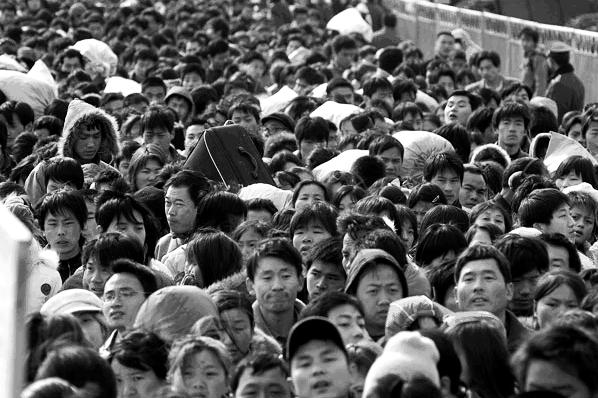
\includegraphics[width=0.4\textwidth]{Figures/history/heat_map_source.jpg}}
	\subfloat[výsledná hustotní mapa]{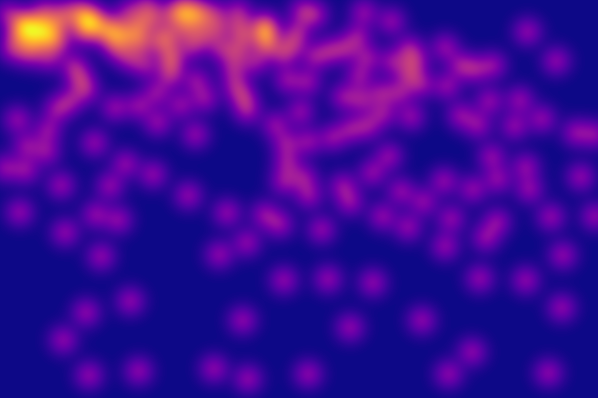
\includegraphics[width=0.4\textwidth]{Figures/history/heat_map.png}}
	\caption{Ukázka hustotní mapy vytvořené pomocí Gausiánů}
\end{figure}

Mezi sítě využívající tento přístup se řadí například M-SFANet \cite{MSFANet_for_crowd_counting}.
Obraz je dán na vstup sítě VGG-16bn \cite{VGG}, která slouží k získání příznaků.
Následně je síť rozdělena na dvě části.
Výstup z desáté vrstvy VGG je dán na vstup modulu CAN (Context-aware module) \cite{CAN_1, CAN_2}, který slouží z získání "scale-aware" příznaků a učí se jejich význam na základě jeho polohy v obraze, což pomáhá, je-li velikost lidí ve vstupním obraze výrazně ovlivněna perspektivou.
Výstup z třinácté vrstvy VGG je vložen na vstup ASPP \cite{ASPP} (Atrous spatial pyramid pooling) modulu, který podobně jako CAN slouží k extrakci "multi scale" příznaků, avšak narozdíl od CAN je jejich důležitost napříč celým obrazem stejná.
Výstupy z těchto modulů jsou vloženy do dvou dekodérů, které slouží vytvoření hustotní a pozornostní mapy (attention map).
Hustotní mapa je vytvořena stejně, jako již výše popsaná, a pozornostní mapa je vytvořena tak, že je-li hodnota v hustotní mapě hodnota větší, než práh, který je stanovený na hodnotu 0,001, tak je hodnota v pozornostní mapě rovna 1, jinak je hodnota rovna 0.
Výsledná hustotní mapa je rovna Hadamardově součinu těchto dvou map.

\begin{figure}[h!]
	\centering
	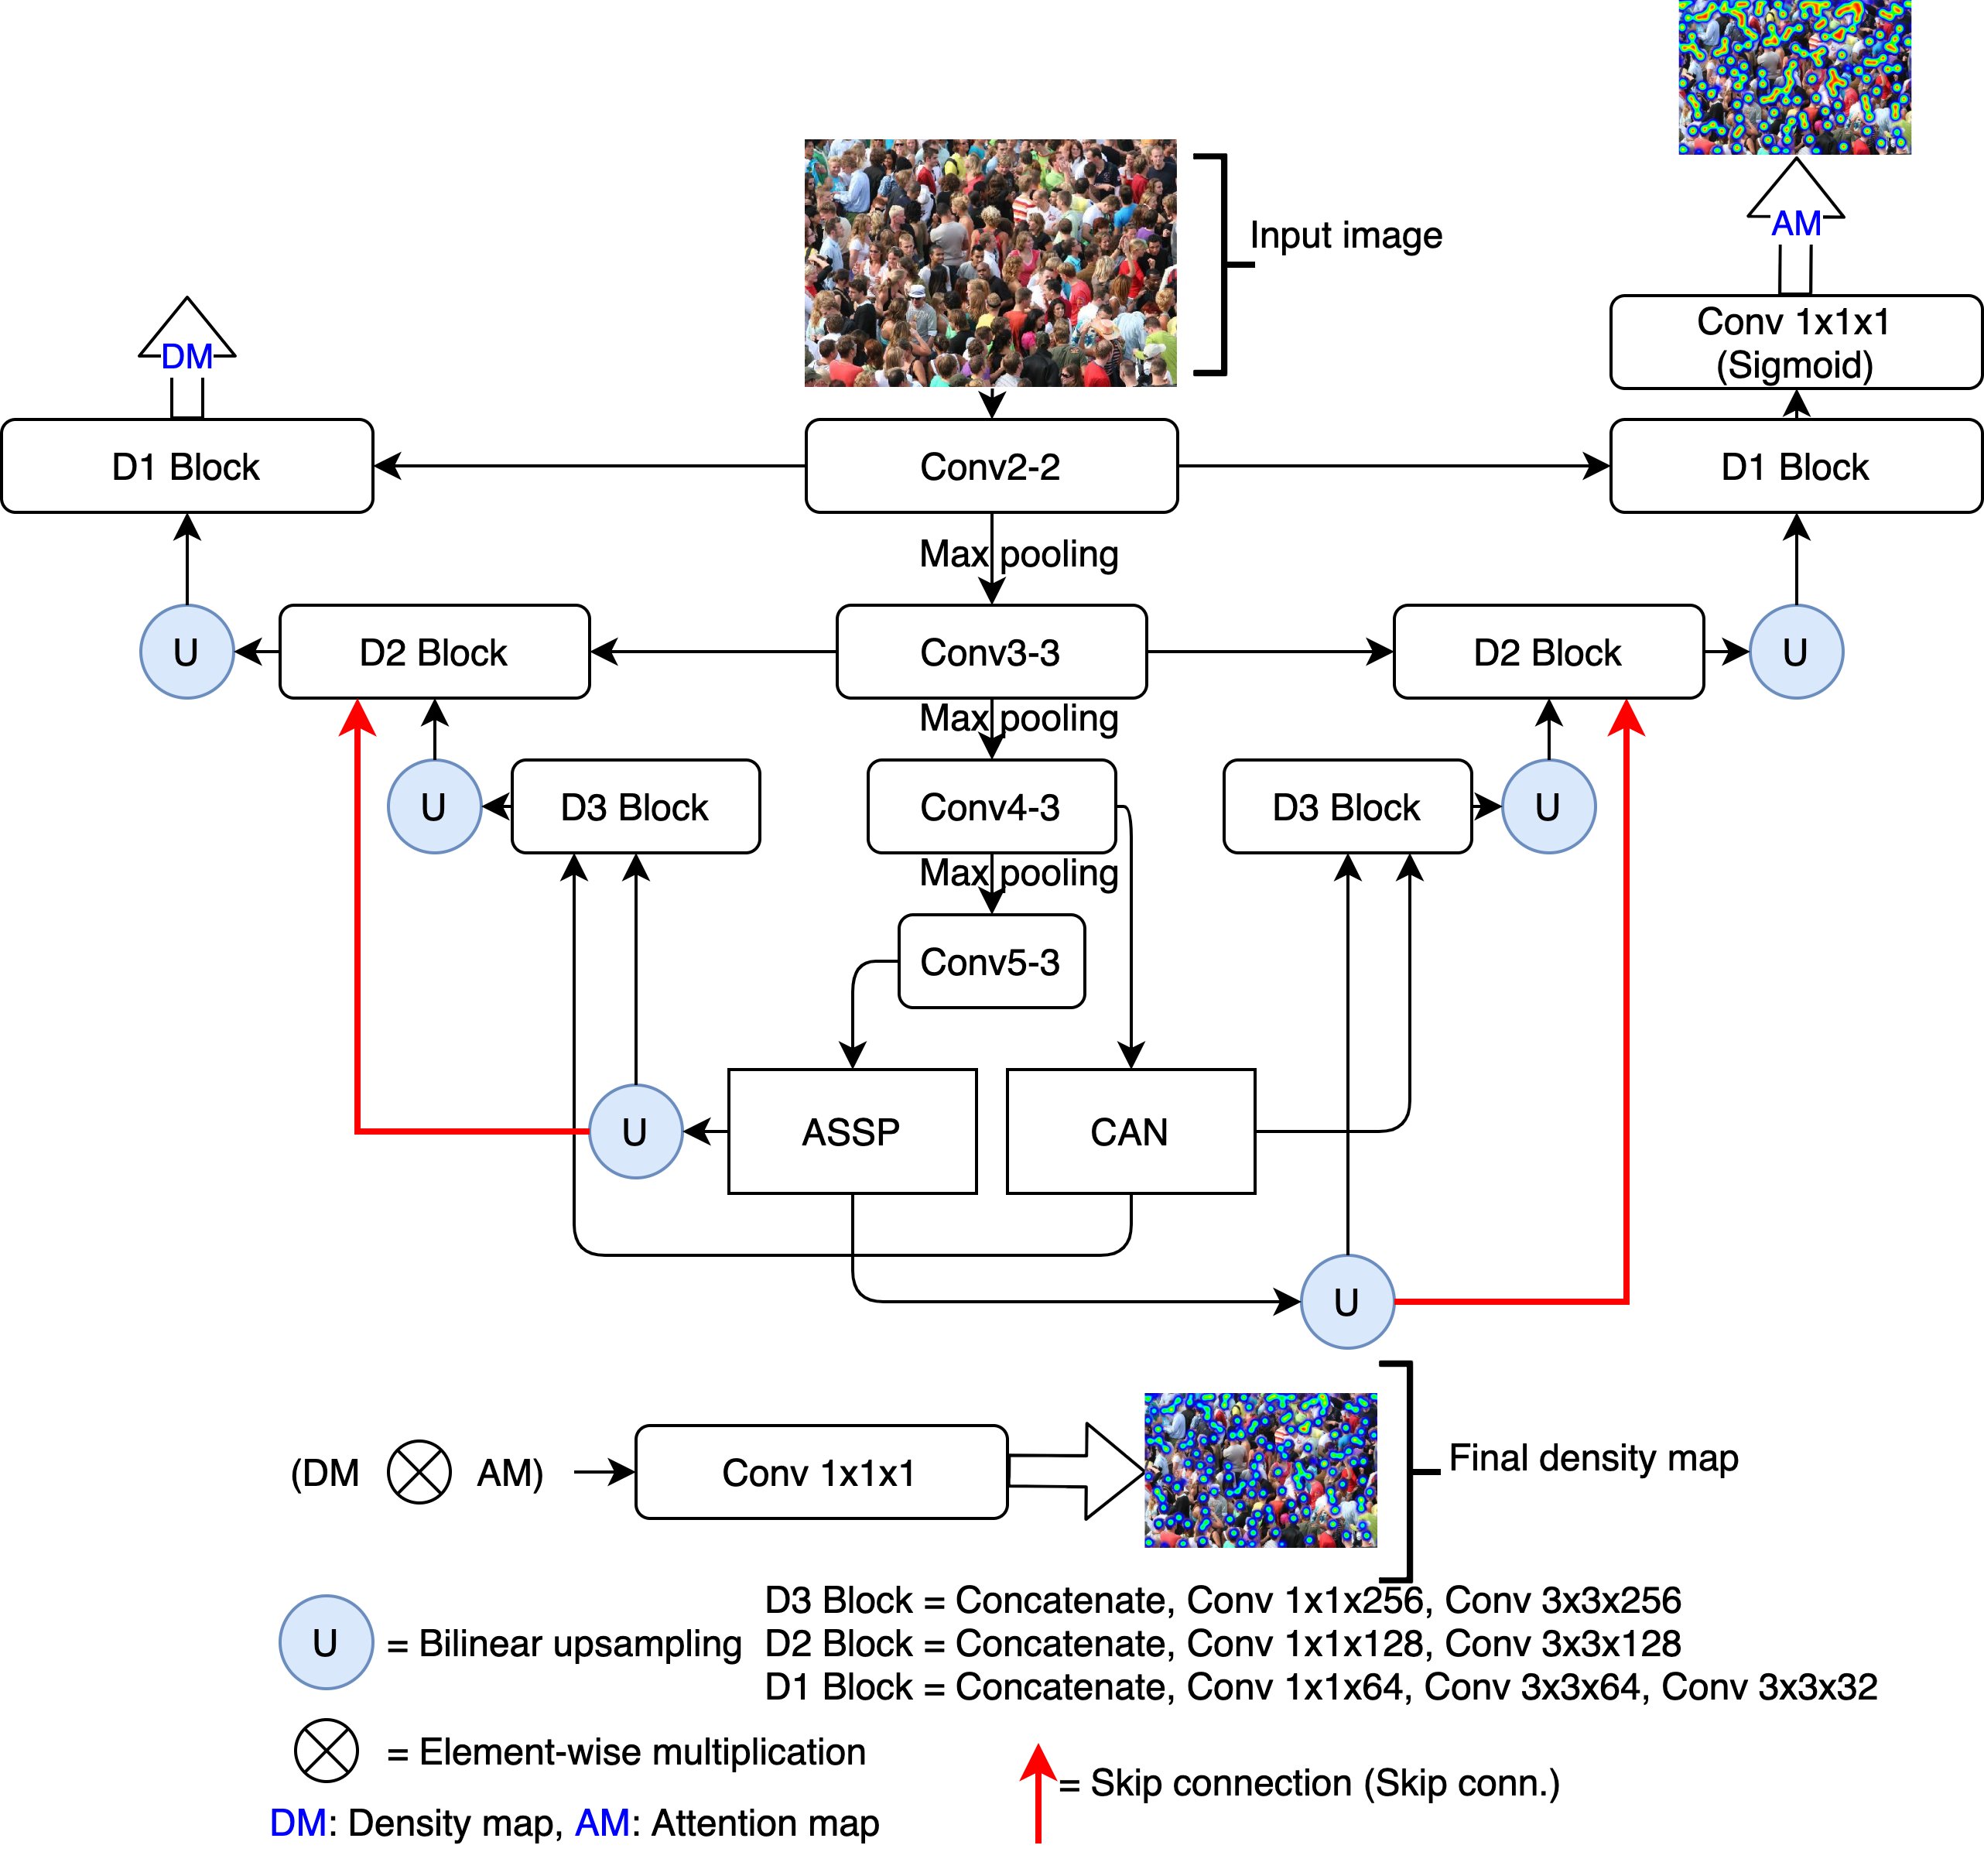
\includegraphics[width=0.6\textwidth]{Figures/history/MSFANet.png}
	\caption{Struktura sítě M-SFANet (převzato z \cite{MSFANet_for_crowd_counting})}
	\label{fig:M-SFANet}
\end{figure}







\endinput